% The MIT License (MIT)
% =====================

% **Copyright (c) 2018 Anish Athalye (me@anishathalye.com)**

% Permission is hereby granted, free of charge, to any person obtaining a copy of
% this software and associated documentation files (the "Software"), to deal in
% the Software without restriction, including without limitation the rights to
% use, copy, modify, merge, publish, distribute, sublicense, and/or sell copies
% of the Software, and to permit persons to whom the Software is furnished to do
% so, subject to the following conditions:

% The above copyright notice and this permission notice shall be included in all
% copies or substantial portions of the Software.

% THE SOFTWARE IS PROVIDED "AS IS", WITHOUT WARRANTY OF ANY KIND, EXPRESS OR
% IMPLIED, INCLUDING BUT NOT LIMITED TO THE WARRANTIES OF MERCHANTABILITY,
% FITNESS FOR A PARTICULAR PURPOSE AND NONINFRINGEMENT. IN NO EVENT SHALL THE
% AUTHORS OR COPYRIGHT HOLDERS BE LIABLE FOR ANY CLAIM, DAMAGES OR OTHER
% LIABILITY, WHETHER IN AN ACTION OF CONTRACT, TORT OR OTHERWISE, ARISING FROM,
% OUT OF OR IN CONNECTION WITH THE SOFTWARE OR THE USE OR OTHER DEALINGS IN THE
% SOFTWARE.


% Gemini theme
% https://github.com/anishathalye/gemini

\documentclass[final]{beamer}

% ====================
% Packages
% ====================

\usepackage[T1]{fontenc}
\usepackage{lmodern}
\usepackage[size=custom,width=130 ,height=100,scale=1.0]{beamerposter}
\usetheme{gemini}
\usecolortheme{gemini}
\usepackage{graphicx}
\usepackage{booktabs}
\usepackage{tikz}
\usepackage{pgfplots}
\usepackage{tcolorbox}
\usepackage{geometry}

% ====================
% Lengths
% ====================

% If you have N columns, choose \sepwidth and \colwidth such that
% (N+1)*\sepwidth + N*\colwidth = \paperwidth
\newlength{\sepwidth}
\newlength{\colwidth}
\setlength{\sepwidth}{0.025\paperwidth}
\setlength{\colwidth}{0.3\paperwidth}

\newcommand{\separatorcolumn}{\begin{column}{\sepwidth}\end{column}}

% ====================
% Title
% ====================

\title{Developing a QIIME 2 plugin - a Simple Annotation for Robust Tools}

\author{Christopher R. Keefe \and Evan Bolyen \textsuperscript{†} \and Matthew Ryan Dillon \textsuperscript{†} \and J. Gregory Caporaso \textsuperscript{†} }

\institute[shortinst]{The Pathogen and Microbiome Institute at Northern Arizona University \\
{\footnotesize \textsuperscript{†} Advisors} }

% ====================
% Body
% ====================

\begin{document}

\begin{frame}[t]
\begin{columns}[t]
\separatorcolumn

\begin{column}{\colwidth}

  \begin{block}{Objective and Introduction}

    \textbf{Objective:} To provide a high-level introduction to the process and
     benefits of developing a  QIIME 2 \cite{10.7287/peerj.preprints.27295v1}
     plugin for computational methods for microbiome science.
    \hfill\break

    \textbf{Introduction:} By wrapping a script in a python 3 package, then
    annotating it with citation/authorship information and information about
    the commands it makes available, the parameters they expose, and the types
    of data they take in and put out, a plugin author can take advantage of
    existing QIIME 2 infrastructure. This can greatly increase the robustness
    and accessibility of their script, improve distribution and citation, and
    facilitate the incorporation of their method into new and existing
    analytical pipelines.
    \hfill\break

    \textbf{QIIME 2 provides:}
    \begin{itemize}
      \item Interfaces: Familiar and powerful user interfaces for a diverse
      user base (e.g. API, command line, graphical, galaxy, cwl)
      \item Community: A vibrant user base, free forum infrastructure for
      plugin support
      \item Visibility: Centralized plugin publishing through the QIIME 2
      Library
      \item Provenance: Integrated and automatic tracking of data provenance,
      and built-in citation support
      \item Low-level infrastructure: facilitates data I/O, communication
      between disparate methods within an analytical pipeline, and
      cross-platform software use
      \item Semantic typing: A rich and extensible type system prevents user
      error, supports backwards compatability and collaboration
      \item Sharing: Allows secure interaction with QIIME 2 artifacts and
      visualizations without a software installation
    \end{itemize}
  \end{block}

  \begin{block}{Develop a method or algorithm}

  In order to develop a QIIME 2 plugin, you must first have code you would
  like to run in QIIME 2. Your method may be written Python 3, or in any
  language accessible to Python 3 with a sub-process call: popular plugins wrap
  code written in R and C, and many options exist.\\
  \hfill\break
  Example: the q2\_alignment plugin wraps the MAFFT application by importing \code{subprocess}, generating input and output filepaths, building a command for the OS from user parameters, and using that command to run MAFFT.\\
      \begin{tcolorbox}
    [width=\textwidth, colframe=blue]
      {
{\texttt{\textcolor{codeblack}{
import subprocess\\
from q2\_types.feature\_data import DNAFASTAFormat, AlignedDNAFASTAFormat\\
\begin{tabbing}
def \=maff\=t(se\=quences: DNAFASTAFormat,\\
\>\>n\_threads: int = 1,\\
\>\>parttree: bool = False) -> AlignedDNAFASTAFormat:\\
\>unaligned\_filepath = str(sequences.path)\\
\>result = AlignedDNAFASTAFormat()\\
\>aligned\_filepath = str(result.path)\\
\\
\>cmd = ["\=mafft", "--preservecase", "--inputorder",\\
\>\>\>"--thread", str(n\_threads), unaligned\_filepath]\\
\\
\>with open(aligned\_filepath, 'w') as output\_f:\\
\>\>subprocess.run(cmd, stdout=output\_f, check=True)
\end{tabbing}}}}
      }
    \end{tcolorbox}

  For the remainder of this poster, we will work with code examples from
  \code{q2-diversity-lib}, a plugin in development for release with QIIME 2 2019.4
  \end{block}

  \begin{block}{Annotate your method}
    QIIME 2 visualizations can be shared and viewed without a software
    install, and contain complete provenance information.

    \begin{enumerate}
      \item Interactive visualizations are significant in understanding and
      communicating our data. (Figure \ref{fig:taxabar-plot})
      \item QIIME 2's provenance graphs allow us to review which methods and
      parameters were used, simplifying creation of an accurate methods section
      and supplementary materials for academic publications.
      \item We can generate a citation list for any result in this poster with \code{qiime tools citations}
      \item Collaborators and reviewers of our work can use https://view.qiime2.org to confirm methods and outcomes are
      appropriate, without the need to download any special software. (Figure 6)
    \end{enumerate}

  \begin{tcolorbox}
  [width=\textwidth, colframe=blue]
  {By packaging \code{Result}s with provenance, QIIME 2 reduces the risk that the
  methods used to produce a given outcome are accidentally misreported.
  QIIME 2 has integrated citation information into plugins, allowing
  researchers to export citations as BibTeX}.
  \end{tcolorbox}

\end{block}

\end{column}

\separatorcolumn

\begin{column}{\colwidth}

  \begin{block}{Introduce new kinds of data}
    Some computational methods require the creation of novel data formats, or
    entirely new types of data. By defining these as Semantic Types in your plugin,
    you allow other QIIME 2 plugins to recognize and use your new data types effectively.

    \begin{tcolorbox}
    [width=\textwidth, colframe=blue]
    {NOTE: The creation of new Semantic Types is a great opportunity for collaboration
    with other developers in the field. Well-architected Types benefit analytical pipeline
    development, and help improve QIIME 2's "understanding" of microbiome data. Further,
    a clear understanding of the Types your method interacts with can clarify and improve the method
    development process.}
    \end{tcolorbox}
  \end{block}

  \begin{block}{Visualizations}
    \begin{figure}[tph!]
    {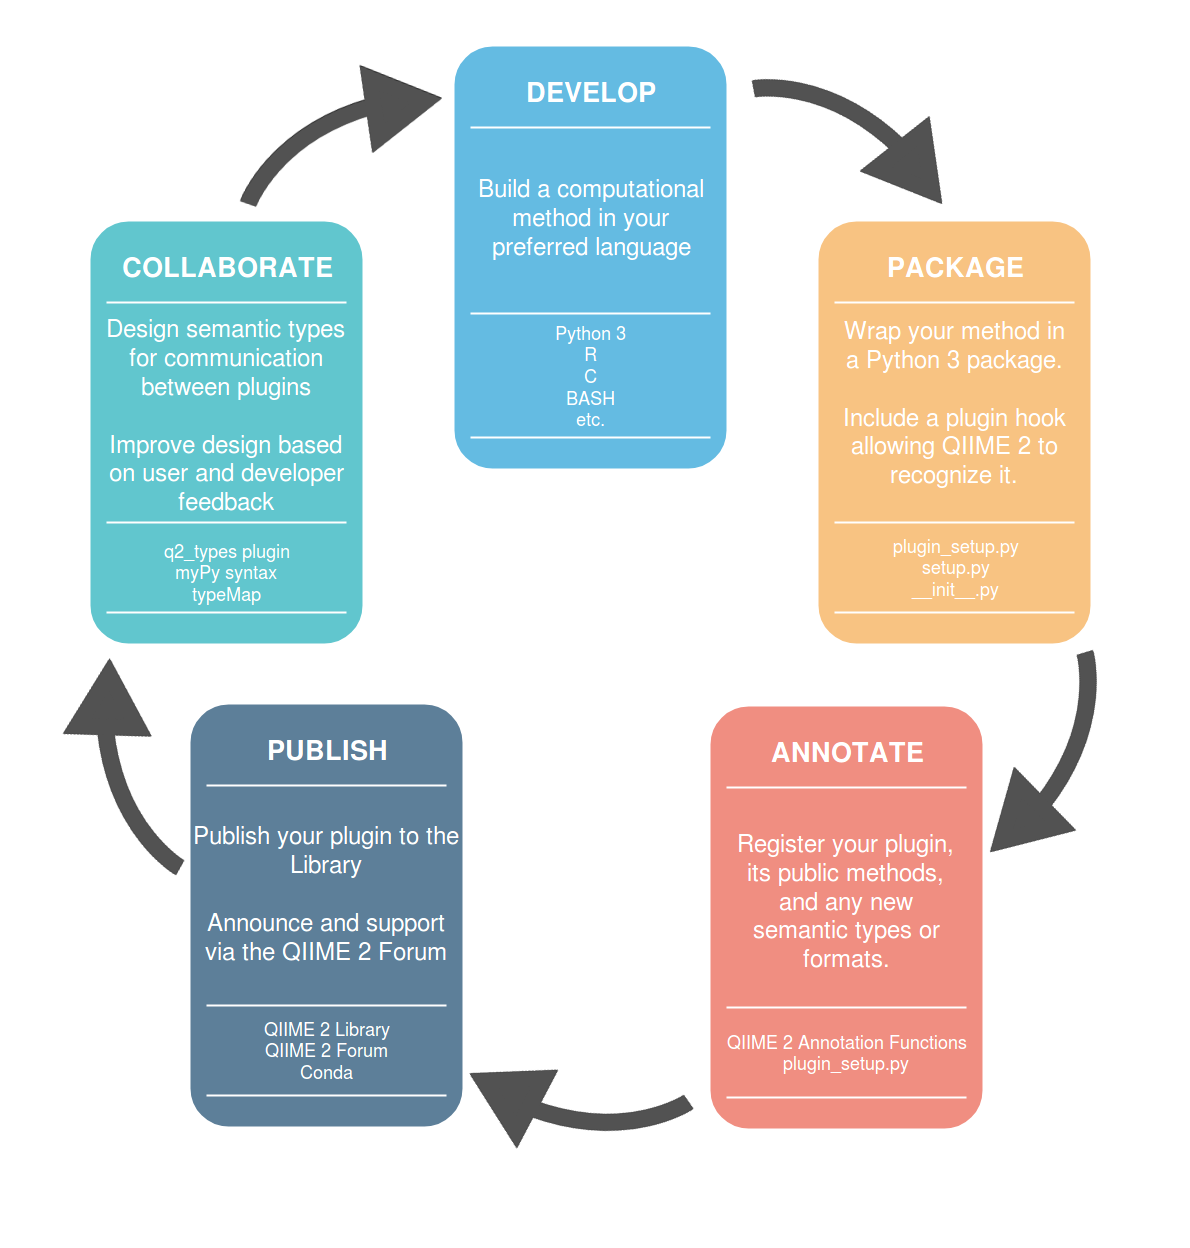
\includegraphics[height=24cm]{assets/DevelopmentProcessDiagramGreyWBG}}
    \caption{\,QIIME 2 plugin development cycle diagram. }
    \label{fig:taxabar-plot}
    \end{figure}

    \begin{figure}[tph!]
    {\includegraphics[height=14cm]{assets/provenance}}
    \caption{\,Provenance tree describing the production of a taxonomic bar plot visualization. Provenance is automatically packaged with ever QIIME 2 Artifact. QR code provides interactive access to provenance tree and bar plot.}
    \label{fig:provenance}
    \end{figure}

    \begin{figure}[tph!]
      {\includegraphics[height=18cm]{assets/q2studio}}
      \caption{\,QIIME 2 Studio provides GUI access to all QIIME 2 plugins installed in the currently active QIIME 2 environment}
      \label{fig:q2studio}
      \end{figure}
  \end{block}

  \begin{block}{Project Funding}
      \begin{figure}[!htb]
        \minipage{0.31\textwidth}%
          \begin{center}
            
\includegraphics[width=.35\linewidth]{assets/SponsorLogos/ABOR}
          \end{center}
        \endminipage
        \hskip 2cm
        \minipage{0.31\textwidth}
          \begin{center}
            
\includegraphics[width=.42\linewidth]{assets/SponsorLogos/APSloanFdn}
          \end{center}
        \endminipage\hfill
        \minipage{0.31\textwidth}
          \begin{center}
            
\includegraphics[width=.50\linewidth]{assets/SponsorLogos/NSF}
          \end{center}
        \endminipage\hfill
      \end{figure}
  \end{block}
\end{column}

\separatorcolumn

\begin{column}{\colwidth}

  \begin{block}{Create a python package}

    Plugins are python packages with metadata hooks which QIIME 2 uses to facilitate
    communication with the other plugins in a given deployment. Packaging
    provides the added benefit of making plugin installation easy for users:

    \begin{figure}[tph!]
      {\includegraphics[height=16cm]{assets/HPC_Analysis}}
      \caption{\,TODO: Diagram like the MAKE THE REPO diagram in Claire's walkthrough}
      \label{fig:dada2}
    \end{figure}

    \begin{tcolorbox}
    [width=\textwidth, colframe=blue]
    {Python packaging may be the most challenging part of plugin creation
    for new developers, because the structure of your software will dictate
    the structure of the package you build. }
    \end{tcolorbox}
    TODO: Reference the tree above\\
    General guidelines:
    \begin{itemize}
      \item Define one or more Python 3 functions, installable with \code{setuptools}
      \item In your \code{plugin\_setup.py}, instantiate a \code{qiime2.plugin.Plugin} object
      \item In your plugin package's \code{setup.py}, define that instance as an entry point
      \item Include \code{\_\_init\_\_.py} files for every subfolder of your plugin which contains function definitions. Note: some of these \code{\_\_init\_\_.py}
      files will only serve to aggregate and make visible subfolder function names
    \end{itemize}
  \end{block}

  \begin{block}{Publish and support}

    QIIME 2’s decentralized provenance tracking makes it easy for anyone to reproduce our
    computational analysis independently to confirm the quality of our results.
    Should one choose to expand our study, or conduct further research using
    similar methods, provenance graphs provide a “road map”.

  \end{block}

  \begin{block}{Future capabilities}

    \begin{itemize}
      \item \textbf{Allow QIIME 2 to consume provenance:} Reading
      provenance \textit{into} QIIME 2 could allow for computer-assisted
      introspection into research methods, automated transcription of methods
      for publication, and auto-generation of “pipeline” scripts for common workflows.
      \item \textbf{QIIME 2 Studio and HPC:} In the future, we hope that QIIME 2 Studio might interact
      directly with HPC schedulers, to simplify the process of connecting with
      and running computationally-intensive processes remotely.
    \end{itemize}

  \end{block}

  \begin{block}{Further Reading}
    \begin{itemize}
      \item \href{https://dev.qiime2.org/latest/tutorials/first-plugin-tutorial/}{Developing a (QIIME 2) Plugin for Dummies: dev.qiime2.org/latest/tutorials/first-plugin-tutorial/}
      \item \href{https://docs.qiime2.org/2019.1/plugins/developing/}{Developing a QIIME 2 Plugin: docs.qiime2.org/2019.1/plugins/developing/}
      \item \href{https://dev.qiime2.org/latest/storing-data/types/}{Semantic and Primitive Types: dev.qiime2.org/latest/storing-data/types/}
      \item \href{https://library.qiime2.org/}{QIIME 2 Library: library.qiime2.org/}
      \item \href{https://python-packaging.readthedocs.io/en/latest/minimal.html}{Python Packaging: python-packaging.readthedocs.io/en/latest/minimal.html}
    \end{itemize}
  \end{block}

  \begin{block}{References}
    \nocite{*}
    \bibliographystyle{acm}\bibliography{poster}
  \end{block}

  \begin{figure}
    \begin{minipage}[c]{\textwidth}
      \hfill
      
\includegraphics[height=5cm]{assets/repo}
    \end{minipage}
    \begin{minipage}[c]{\textwidth}
      \hfill
      Poster Source: https://github.com/ChrisKeefe/SACMDA19
    \end{minipage}
  \end{figure}

\end{column}

\separatorcolumn
\end{columns}
\end{frame}
\end{document}
